\documentclass[conference]{IEEEtran}
\IEEEoverridecommandlockouts

\usepackage{cite}
\usepackage{amsmath,amssymb}
\usepackage{graphicx}
\usepackage{xcolor}
\usepackage{booktabs}
\usepackage{multirow}
\usepackage{url}
\usepackage{array}
\usepackage{tikz}
\usetikzlibrary{positioning,arrows.meta,shapes.geometric,fit,calc}

\title{Compression-Resilient Deepfake Detection via\\Attentive Spatial--Frequency Fusion}

\author{
\IEEEauthorblockN{Yash Aggarwal \hspace{1.2em} Yash Jain}
\IEEEauthorblockA{Department of Computer Science and Engineering\\
Delhi Technological University, Delhi, India\\
Email: \{yashaggarwal,yashjain\}@dtu.ac.in}
}

\begin{document}
\maketitle

% ================================================================
% ABSTRACT
% ================================================================
\begin{abstract}
Deepfake detection models frequently achieve high in-domain accuracy yet degrade sharply under lossy compression and cross-dataset distribution shifts---the two most common conditions in real-world media pipelines.
We present a dual-stream deepfake detector that fuses spatial RGB features extracted by an Xception backbone with frequency-domain cues derived from per-channel Discrete Cosine Transform (DCT) maps processed by a lightweight ResNet-18 backbone.
A learned 512-dimensional channel-wise gate adaptively blends the two representations, enabling the model to down-weight unreliable frequency dimensions when compression destroys high-frequency artifacts.
To further improve robustness, we employ compression-aware training augmentations including JPEG simulation, resolution degradation, and frequency-domain masking.
We evaluate under a transparent operating-point protocol: thresholds are selected on an internal FaceForensics++ validation split and applied to cross-dataset Celeb-DF-v2 testing.
We report both threshold-free metrics (AUROC, Average Precision) and operating-point metrics (EER, TPR@FPR, balanced accuracy).
Our model achieves a video-level AUROC of 0.9955 in-domain and 0.9018 cross-dataset on Celeb-DF-v2.
Under aggressive JPEG compression (QF\,=\,20), the in-domain AUROC degrades gracefully from 0.9956 to 0.9396, a relative drop of only 5.6\%.
Under the combined stress of compression and domain shift (Celeb-DF-v2 at QF\,=\,20), AUROC remains at 0.820, demonstrating practical resilience.
Ablation experiments confirm that fusing frequency features with the spatial stream improves over the spatial-only baseline.
\end{abstract}

\begin{IEEEkeywords}
Deepfake detection, face forgery, frequency domain, DCT, cross-dataset generalization, compression robustness, AUROC, gated fusion
\end{IEEEkeywords}

% ================================================================
% 1. INTRODUCTION
% ================================================================
\section{Introduction}

\textbf{Motivation.}
Rapid advances in face synthesis and reenactment have made it possible to produce highly realistic manipulated videos, commonly termed \emph{deepfakes}.
Their potential for political disinformation, identity fraud, and non-consensual pornography has motivated a growing body of work on automated deepfake detection~\cite{rossler2019faceforensics,li2020celebdf}.

\textbf{Problem statement.}
Although many detectors report near-perfect in-domain accuracy, two systemic weaknesses limit practical deployment:
(i)~\emph{Compression fragility}---social media and messaging platforms re-encode uploaded videos with aggressive lossy codecs (JPEG, H.264/H.265), which preferentially destroys the high-frequency forensic traces that many detectors rely on~\cite{frank2020leveraging};
(ii)~\emph{Cross-dataset generalization}---detectors overfit to dataset-specific artifacts (e.g., blending boundaries, colour distributions) and fail when exposed to unseen generators or post-processing pipelines~\cite{li2020facexray,yan2023ucf,wang2024wilddeepfake}.

\textbf{Challenges.}
Frequency-domain features are powerful discriminators under controlled conditions~\cite{qian2020f3net,durall2020watch}, yet they are the first casualties of lossy compression.
Purely spatial detectors are more resilient to compression but may latch onto dataset-level shortcuts, reducing generalization.
A further challenge is \emph{evaluation bias}: reporting accuracy at a fixed threshold of 0.5 on imbalanced datasets (e.g., Celeb-DF-v2 with a 9.5:1 fake-to-real ratio) can paint a misleadingly optimistic picture.

\textbf{Contributions.}
\begin{itemize}
  \item We design a dual-stream architecture that combines Xception~\cite{chollet2017xception} spatial features with ResNet-18~\cite{he2016resnet} frequency features through a learned 512-D channel-wise gate, enabling fine-grained per-dimension control over spatial vs.\ frequency reliance.
  \item We integrate compression-aware training augmentations---JPEG simulation, resolution degradation, Gaussian blur, colour jitter, and frequency-domain masking---to reduce sensitivity to compression artifacts.
  \item We adopt a transparent evaluation protocol: thresholds are selected on a held-out validation split, and both threshold-free (AUROC, AP) and operating-point metrics (EER, TPR@FPR, balanced accuracy) are reported.
  \item We provide a systematic robustness analysis: JPEG quality-factor sweeps, cross-dataset evaluation, ablation studies, and Grad-CAM visualizations.
\end{itemize}

% ================================================================
% 2. RELATED WORK
% ================================================================
\section{Related Work}

\subsection{Deepfake Detection Methods}
Early approaches used handcrafted cues such as eye-blink inconsistencies~\cite{li2018ictu}. CNN-based methods later became dominant, with Xception~\cite{chollet2017xception,rossler2019faceforensics} and EfficientNet~\cite{tan2019efficientnet} establishing strong baselines.
Face X-ray~\cite{li2020facexray} detects blending boundaries, while SBI~\cite{shiohara2022sbi} uses self-blended images for augmentation.
Multi-Attentional~\cite{zhao2021multiattentional} localizes tampered regions with texture attention, and RECCE~\cite{cao2022recce} employs reconstruction-classification learning.
More recently, UCF~\cite{yan2023ucf} uncovers common forgery features shared across manipulation methods to improve cross-dataset generalization, while TALL~\cite{xu2023tall} exploits temporal thumbnail layouts for video-level detection.
Implicit identity cues have also been leveraged for face-swap detection~\cite{dong2023implicit}.
Vision-language alignment has emerged as a promising direction~\cite{sun2024towards}, and fairness-aware training strategies address demographic bias in detectors~\cite{lin2024preserving}.
For a comprehensive survey of the field through 2025, see Zhang~et~al.~\cite{zhang2025survey}.

\subsection{Frequency-Domain Cues}
Frank~et~al.~\cite{frank2020leveraging} demonstrated that GAN-generated images exhibit characteristic spectral artefacts.
Durall~et~al.~\cite{durall2020watch} showed that up-convolution layers fail to reproduce natural spectral distributions.
F3-Net~\cite{qian2020f3net} mines frequency-aware clues via learnable frequency filters, and SPSL~\cite{liu2021spsl} rethinks detection in the phase spectrum.
SRM~\cite{luo2021hf} uses high-frequency features for generalization.
Our work differs in that we explicitly model the \emph{reliability} of frequency features through a learned per-dimension gate, rather than relying on a fixed fusion strategy.

\subsection{Compression Robustness and Cross-Dataset Generalization}
Real-world media undergo aggressive lossy encoding, destroying high-frequency forensic traces.
Wang~et~al.~\cite{wang2022m2tr} proposed multi-modal transformers for robustness, while AltFreezing~\cite{wang2023altfreezing} alternates spatial and temporal learning for video-level robustness.
LAA-Net~\cite{nguyen2024laanet} localizes artefacts for quality-agnostic and compression-resilient detection.
LSDA~\cite{chen2024lsda} scales training data to improve generalization across unseen generators, and forgery-aware transformers~\cite{liu2024forgery} adapt to novel synthesis methods without retraining.
Controllable guide-space methods~\cite{guo2023controllable} disentangle identity from forgery features to reduce domain sensitivity.
WildDeepfake~\cite{wang2024wilddeepfake} provides a challenging in-the-wild benchmark that highlights the performance gap between controlled evaluation and real deployment conditions.
Our approach addresses compression robustness through both architectural design (adaptive gating) and training strategy (JPEG-aware augmentations).

% ================================================================
% 3. METHODOLOGY
% ================================================================
\section{Methodology}

\subsection{Architecture Overview}
Given an input face crop $I \in \mathbb{R}^{H \times W \times 3}$, our detector processes it through two parallel streams and a gated fusion module (Fig.~\ref{fig:arch}):

\begin{figure*}[t]
  \centering
  \resizebox{\textwidth}{!}{%
  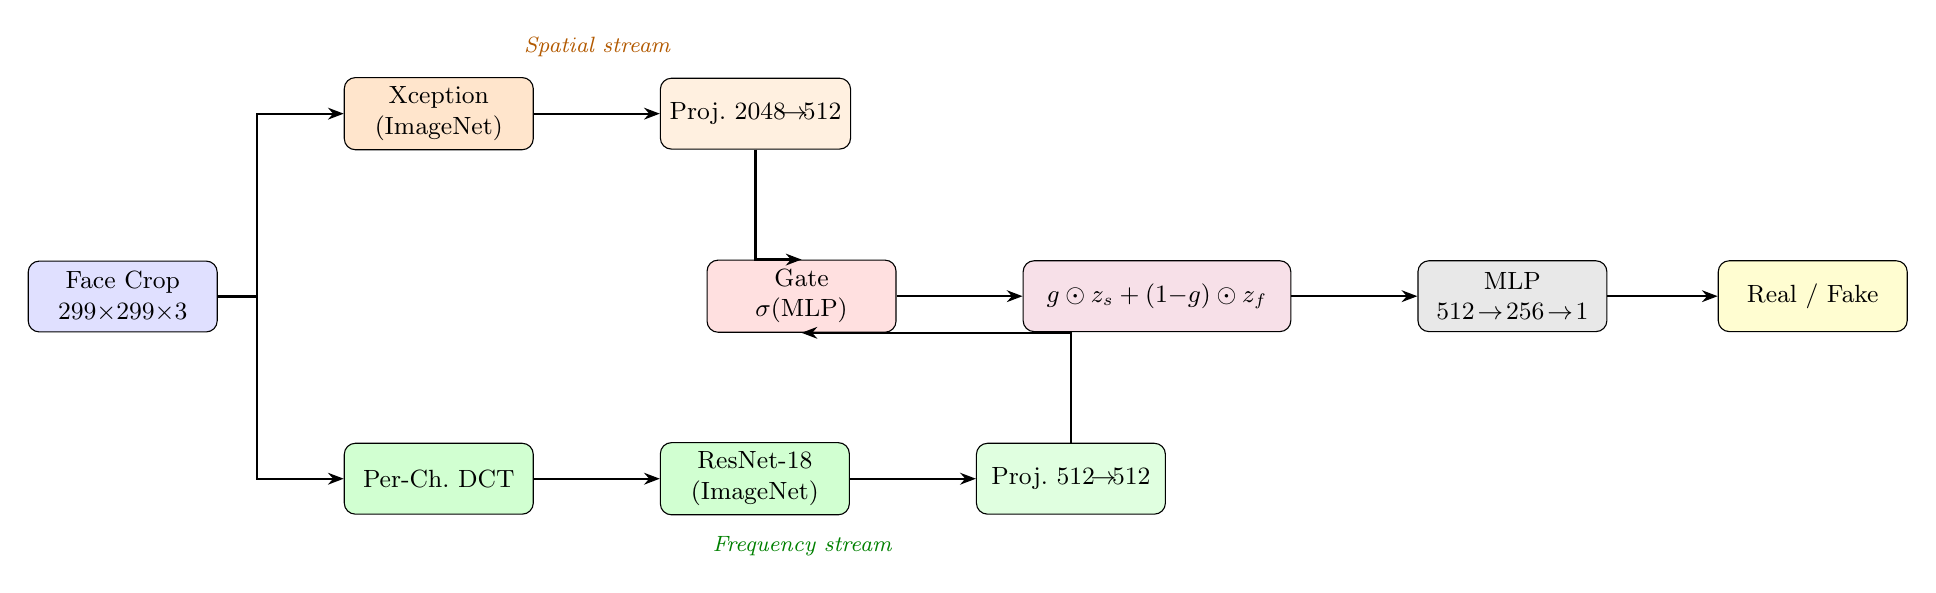
\begin{tikzpicture}[
      block/.style={draw, rounded corners, minimum height=0.9cm, minimum width=2.4cm,
                    align=center, font=\small},
      wideblock/.style={draw, rounded corners, minimum height=0.9cm, minimum width=3.4cm,
                    align=center, font=\small},
      arrow/.style={-{Stealth[length=2mm]}, thick},
      darrow/.style={-{Stealth[length=2mm]}, thick, dashed, gray},
      node distance=0.6cm and 1.6cm
  ]
  
  %% ---- Input ----
  \node[block, fill=blue!12] (input) {Face Crop\\$299{\times}299{\times}3$};
  
  %% ---- Spatial stream (top) ----
  \node[block, fill=orange!20, above right=1.4cm and 1.6cm of input] (xception)
      {Xception\\(ImageNet)};
  \node[block, fill=orange!12, right=1.6cm of xception] (s_proj)
      {Proj.\ 2048$\!\to\!$512};
  
  %% ---- Frequency stream (bottom) ----
  \node[block, fill=green!18, below right=1.4cm and 1.6cm of input] (dct)
      {Per-Ch.\ DCT};
  \node[block, fill=green!18, right=1.6cm of dct] (resnet)
      {ResNet-18\\(ImageNet)};
  \node[block, fill=green!12, right=1.6cm of resnet] (f_proj)
      {Proj.\ 512$\!\to\!$512};
  
  %% ---- Gate (vertically centered between the two streams) ----
  \node[block, fill=red!12] (gate) at ($(xception)!0.5!(resnet)+(2.6,0)$)
      {Gate\\$\sigma$(MLP)};
  
  %% ---- Fusion (to the right of gate) ----
  \node[wideblock, fill=purple!12, right=1.6cm of gate] (fusion)
      {$g \odot z_s + (1{-}g) \odot z_f$};
  
  %% ---- Classifier ----
  \node[block, fill=gray!18, right=1.6cm of fusion] (mlp)
      {MLP\\$512\!\to\!256\!\to\!1$};
  \node[block, fill=yellow!18, right=1.4cm of mlp] (out)
      {Real / Fake};
  
  %% ---- Connections ----
  
  % Input to spatial and frequency streams
  \draw[arrow] (input.east) -- ++(0.5,0) |- (xception.west);
  \draw[arrow] (input.east) -- ++(0.5,0) |- (dct.west);
  
  % Spatial stream internal
  \draw[arrow] (xception) -- (s_proj);
  
  % Frequency stream internal
  \draw[arrow] (dct) -- (resnet);
  \draw[arrow] (resnet) -- (f_proj);
  
  % s_proj and f_proj → Gate (vertical arrows into top/bottom of gate)
  \draw[arrow] (s_proj.south) |- (gate.north);
  \draw[arrow] (f_proj.north) |- (gate.south);
  
  % Gate → Fusion (gate values g)
  \draw[arrow] (gate.east) -- (fusion.west);
  
  % Fusion → MLP → Output
  \draw[arrow] (fusion) -- (mlp);
  \draw[arrow] (mlp) -- (out);
  
  %% ---- Stream Labels ----
  \node[font=\footnotesize\itshape, text=orange!70!black]
      at ($(xception)!0.5!(s_proj)+(0,0.85)$) {Spatial stream};
  \node[font=\footnotesize\itshape, text=green!50!black]
      at ($(dct)!0.5!(f_proj)+(0.6,-0.85)$) {Frequency stream};
  
  \end{tikzpicture}
  }
  \caption{Dual-stream architecture. The spatial stream (Xception) and frequency stream
  (ResNet-18 on DCT coefficients) are each projected to a shared 512-D space.
  A learned gating module $\sigma(\text{MLP})$ produces a soft gate $g$ that blends
  the two feature vectors before a final MLP classifier outputs Real/Fake.}
  \label{fig:arch}
  \end{figure*}

\begin{table}[t]
\centering
\caption{Architecture specification.}
\label{tab:archspec}
\begin{tabular}{>{\raggedright\arraybackslash}p{0.38\columnwidth} >{\raggedright\arraybackslash}p{0.54\columnwidth}}
\toprule
\textbf{Component} & \textbf{Details} \\
\midrule
Spatial backbone & Xception, 2048-D output \\
Frequency backbone & ResNet-18 on 3-ch DCT, 512-D output \\
Projections & 2048$\to$512 and 512$\to$512, ReLU \\
Gate network & 1024$\to$512$\to$512, Sigmoid \\
Fusion & $z = g\odot z_s + (1{-}g)\odot z_f$ \\
Classifier & 512$\to$256$\to$1, Dropout 0.5 \\
\midrule
Total parameters & ${\sim}$35.2\,M \\
\bottomrule
\end{tabular}
\end{table}

\subsection{Frequency Representation: Per-Channel DCT}
Rather than converting the image to grayscale, we compute the 2-D DCT independently for each RGB channel, preserving colour-channel forensic information:
\begin{equation}
  D_c(u,v) = \log\!\bigl(|{\rm DCT}\{I_c\}(u,v)| + \epsilon\bigr), \quad c\in\{R,G,B\},
  \label{eq:dct}
\end{equation}
where $\epsilon=10^{-6}$ stabilizes the logarithm. Each channel is min-max normalized independently. Because JPEG and MPEG operate in DCT-like domains, this representation provides a natural interface for capturing compression-related artefacts and generator-specific spectral signatures.

\subsection{Channel-Wise Gated Fusion}
Instead of assigning a single scalar weight per stream, we learn a 512-dimensional gate conditioned on the concatenated projected features:
\begin{equation}
  g = \sigma\!\bigl(\mathrm{MLP}([z_s;\, z_f])\bigr) \in (0,1)^{512},
  \label{eq:gate}
\end{equation}
\begin{equation}
  z = g \odot z_s + (1{-}g) \odot z_f.
  \label{eq:fusion}
\end{equation}
This enables fine-grained control per feature dimension: under heavy compression, the model can down-weight unstable frequency dimensions while preserving robust spatial cues.

\subsection{Training Configuration}

\textbf{Loss function.}
We use Focal Loss~\cite{lin2017focal} with $\alpha=0.25$, $\gamma=2.0$ to focus on hard examples:
\begin{equation}
  \mathcal{L}_{\rm focal} = -\alpha\,(1{-}p_t)^{\gamma}\log(p_t).
\end{equation}

\textbf{Optimization.}
AdamW~\cite{loshchilov2019adamw} with learning rate $10^{-4}$, weight decay $10^{-4}$, cosine annealing warm restarts~\cite{loshchilov2017sgdr} ($T_0{=}5$, $T_{\rm mult}{=}2$), gradient clipping at norm 1.0, and label smoothing ($\epsilon{=}0.05$).
Training runs for up to 10 epochs with early stopping (patience\,=\,7) based on validation AUROC.

\begin{table}[t]
\centering
\caption{Training hyperparameters.}
\label{tab:hparams}
\begin{tabular}{ll}
\toprule
\textbf{Hyperparameter} & \textbf{Value} \\
\midrule
Input resolution & $299\times299$ \\
Batch size & 32 \\
Optimizer & AdamW ($\beta_1{=}0.9$, $\beta_2{=}0.999$) \\
Learning rate & $1\times10^{-4}$ \\
Weight decay & $1\times10^{-4}$ \\
LR schedule & Cosine Annealing WR \\
Focal Loss ($\alpha$, $\gamma$) & 0.25, 2.0 \\
Label smoothing & 0.05 \\
Gradient clipping & 1.0 \\
Early stopping patience & 7 epochs \\
\bottomrule
\end{tabular}
\end{table}

\subsection{Compression-Aware Augmentations}
During training, we apply the following augmentations stochastically to each sample:
\begin{itemize}
  \item \textbf{JPEG compression simulation} (40\% probability): encode to an in-memory JPEG buffer at a random quality factor $q\sim\mathcal{U}(30,95)$ and decode, introducing authentic block artefacts and quantization noise.
  \item \textbf{Gaussian blur} (50\%): kernel radius $r\sim\mathcal{U}(0.1,1.5)$.
  \item \textbf{Resolution degradation} (40\%): bicubic downscale by factor $s\sim\mathcal{U}(0.5,0.9)$, then upscale to original resolution.
  \item \textbf{Frequency-domain masking (FDM)} (50\%): randomly zero a rectangular block of up to 15\% of the DCT map, reducing reliance on any single frequency band.
  \item \textbf{Colour jitter}: brightness, contrast, saturation $\pm0.2$; hue $\pm0.05$.
\end{itemize}
Critically, the DCT map is computed \emph{after} spatial augmentations, so the frequency stream observes the compressed/perturbed state of the image.

\subsection{Evaluation Protocol}
\textbf{Operating-point selection.}
We select thresholds on the FF++ validation split using Youden's $J$ statistic ($\arg\max_\theta [\text{TPR}(\theta) - \text{FPR}(\theta)]$) and apply them to all test splits. This avoids the common pitfall of reporting accuracy at a fixed 0.5 threshold on imbalanced datasets.

\textbf{Metrics.}
We report threshold-free metrics (AUROC, Average Precision) and operating-point metrics (Equal Error Rate, TPR@FPR=1\%, TPR@FPR=5\%, balanced accuracy, macro-F1).

\textbf{Video aggregation.}
Frame-level sigmoid probabilities are averaged per video directory to produce video-level scores.

% ================================================================
% 4. DATASETS
% ================================================================
\section{Datasets}

\begin{table}[t]
\centering
\caption{Dataset summary. FF++ includes four manipulation methods; Celeb-DF-v2 is used for cross-dataset testing only.}
\label{tab:datasets}
\begin{tabular}{lcccl}
\toprule
\textbf{Dataset} & \textbf{Videos} & \textbf{Manip.} & \textbf{Compr.} & \textbf{Role} \\
\midrule
FF++~\cite{rossler2019faceforensics} & 5,000 & 4 & c23/c40 & Train + Val \\
Celeb-DF-v2~\cite{li2020celebdf} & 6,229 & 1 & H.264 & Test \\
DFDC~\cite{dolhansky2020dfdc} & 128K & var. & var. & Future \\
\bottomrule
\end{tabular}
\end{table}

\textbf{FaceForensics++ (FF++)}~\cite{rossler2019faceforensics} contains 1,000 original YouTube videos manipulated by four methods: Deepfakes, Face2Face, FaceSwap, and NeuralTextures. We use the c23 (light compression) variant and split into train/validation.

\textbf{Celeb-DF-v2}~\cite{li2020celebdf} provides 590 real and 5,639 fake celebrity videos synthesized with an improved pipeline. Its distribution differs substantially from FF++, making it a challenging cross-dataset benchmark.

\textbf{DFDC}~\cite{dolhansky2020dfdc} contains over 128,000 clips; we reference it as a target for future evaluation.

% ================================================================
% 5. EXPERIMENTAL SETUP
% ================================================================
\section{Experimental Setup}

Faces are detected and cropped from source videos using MTCNN~\cite{zhang2016mtcnn} and resized to $299\times299$.
Both the RGB crop and its per-channel DCT map (Eq.~\ref{eq:dct}) are normalized to $[-1,1]$ and fed to the dual-stream model.
All experiments use a single Apple M-series GPU (MPS backend), batch size 16 at evaluation, and 2 data-loading workers.

% ================================================================
% 6. RESULTS
% ================================================================
\section{Results}

\subsection{In-Domain Performance (FF++ Validation)}
Table~\ref{tab:main_ffpp} summarises frame-level and video-level results on the internal FF++ validation split.
Video-level aggregation consistently improves AUROC, indicating that averaging across frames reduces noise and yields more stable per-video decisions.
The model achieves a video-level AUROC of 0.9955 and balanced accuracy of 0.9751, demonstrating strong in-domain discrimination.

\begin{table}[t]
\centering
\caption{In-domain results on FF++ validation (Youden threshold selected on this split).}
\label{tab:main_ffpp}
\begin{tabular}{lccccc}
\toprule
\textbf{Level} & \textbf{AUROC} & \textbf{AP} & \textbf{EER} & \textbf{BalAcc} & \textbf{F1\textsubscript{macro}} \\
\midrule
Frame & 0.9804 & 0.9969 & 0.069 & 0.934 & 0.852 \\
Video & 0.9955 & 0.9990 & 0.031 & 0.975 & 0.951 \\
\bottomrule
\end{tabular}
\end{table}

\subsection{Cross-Dataset Generalization (Celeb-DF-v2)}
Table~\ref{tab:main_cdf} reports results when the model trained on FF++ is tested on Celeb-DF-v2 with thresholds selected on the FF++ validation split.
The video-level AUROC of 0.9018 reflects a significant but expected drop compared to the in-domain 0.9955, attributable to the domain gap between FF++ and Celeb-DF-v2 generators, preprocessing, and compression pipelines.
Balanced accuracy drops more steeply (from 0.975 to 0.809), highlighting that the threshold optimal for FF++ is suboptimal under domain shift.

\begin{table}[t]
\centering
\caption{Cross-dataset results on Celeb-DF-v2 (thresholds from FF++ validation).}
\label{tab:main_cdf}
\begin{tabular}{lccccc}
\toprule
\textbf{Level} & \textbf{AUROC} & \textbf{AP} & \textbf{EER} & \textbf{BalAcc} & \textbf{F1\textsubscript{macro}} \\
\midrule
Frame & 0.8227 & 0.9752 & 0.260 & 0.737 & 0.559 \\
Video & 0.9018 & 0.9873 & 0.175 & 0.809 & 0.720 \\
\bottomrule
\end{tabular}
\end{table}

Fig.~\ref{fig:roc} shows the ROC curves for both settings, highlighting the area between the in-domain and cross-dataset performance envelopes.

\begin{figure}[t]
  \centering
  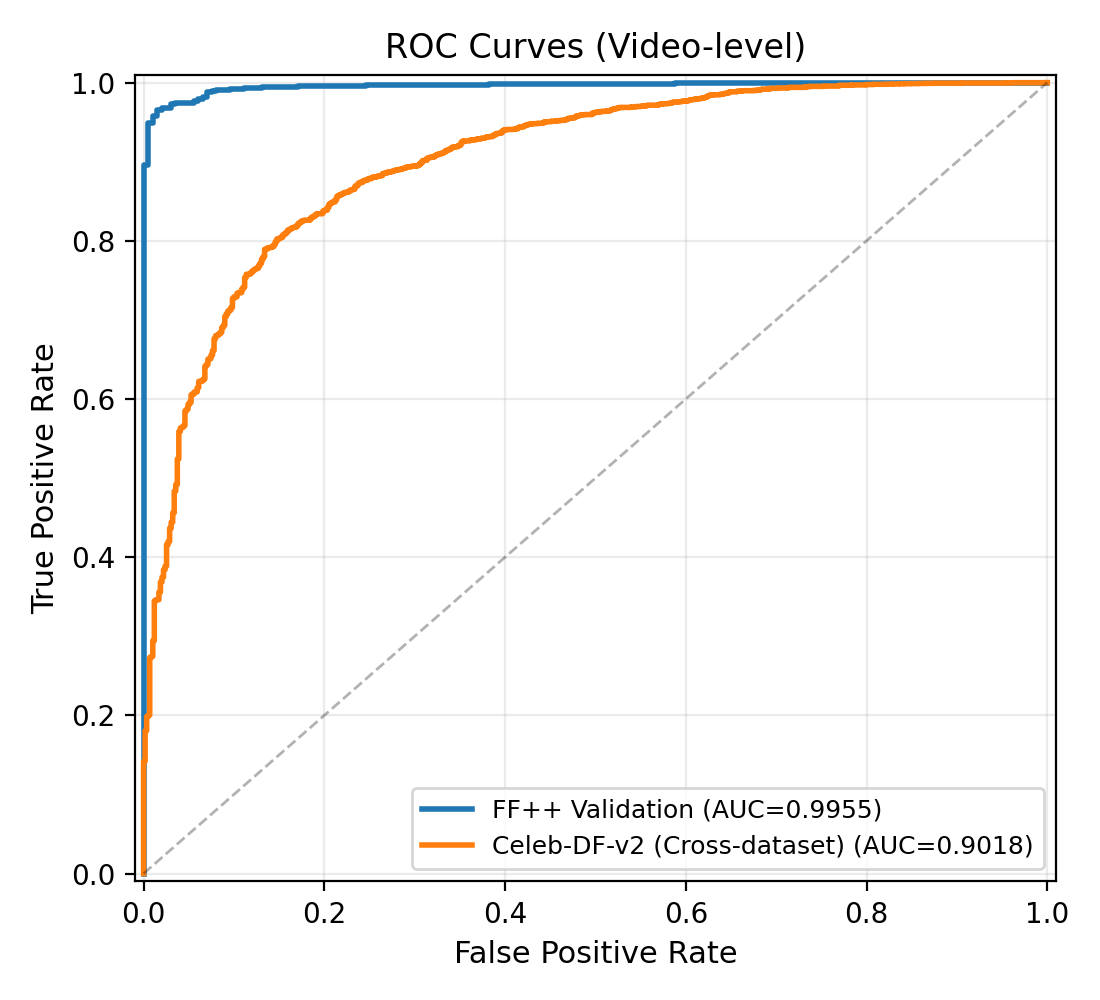
\includegraphics[width=\columnwidth]{figs/roc_combined.png}
  \caption{Video-level ROC curves on FF++ validation (AUC\,=\,0.9955) and Celeb-DF-v2 (AUC\,=\,0.9018).}
  \label{fig:roc}
\end{figure}

\subsection{Operating-Point Analysis}
Table~\ref{tab:operating} compares video-level metrics at four operating points on Celeb-DF-v2.
At a strict FPR=1\% setting, only 27.5\% of fakes are detected---a sharp drop from the 94.9\% achievable at the same operating point in-domain.
This illustrates the standard precision-recall trade-off under domain shift and class imbalance (590 real vs.\ 5,639 fake videos).
The Youden-selected threshold provides a practical balance between false positives and true positives.

\begin{table}[t]
\centering
\caption{Video-level operating-point comparison on Celeb-DF-v2 (thresholds from FF++ validation).}
\label{tab:operating}
\begin{tabular}{lcccc}
\toprule
\textbf{Threshold} & \textbf{$\theta$} & \textbf{BalAcc} & \textbf{Prec\textsubscript{R}} & \textbf{Rec\textsubscript{R}} \\
\midrule
Youden  & 0.716 & 0.809 & 0.397 & 0.736 \\
FPR=1\% & 0.770 & 0.825 & 0.305 & 0.854 \\
FPR=5\% & 0.682 & 0.786 & 0.465 & 0.649 \\
Fixed 0.5 & 0.500 & 0.621 & 0.849 & 0.247 \\
\bottomrule
\end{tabular}
\end{table}

\subsection{Compression Robustness (JPEG Quality Sweep)}
To quantify compression resilience, we JPEG-compress face crops in memory at five quality factors (QF~$\in\{100,80,60,40,20\}$) before inference and report video-level AUROC on the FF++ validation split (Table~\ref{tab:jpeg}, Fig.~\ref{fig:jpeg}).

From QF=100 to QF=20, AUROC drops from 0.9956 to 0.9396---a relative decrease of only 5.6\%.
Balanced accuracy shows a larger decline (from 0.974 to 0.861), since the threshold selected at QF=100 becomes suboptimal as compression increases.
This graceful degradation validates the effectiveness of our compression-aware augmentations and adaptive gating mechanism.

\begin{table}[t]
\centering
\caption{JPEG compression robustness (FF++ validation, video-level).}
\label{tab:jpeg}
\begin{tabular}{cccccc}
\toprule
\textbf{QF} & \textbf{AUROC} & \textbf{AP} & \textbf{EER} & \textbf{BalAcc} & \textbf{TPR@1\%} \\
\midrule
100 & 0.9956 & 0.9990 & 0.030 & 0.974 & 0.934 \\
80  & 0.9934 & 0.9985 & 0.040 & 0.962 & 0.926 \\
60  & 0.9872 & 0.9971 & 0.059 & 0.946 & 0.868 \\
40  & 0.9759 & 0.9943 & 0.075 & 0.925 & 0.729 \\
20  & 0.9396 & 0.9853 & 0.140 & 0.861 & 0.533 \\
\bottomrule
\end{tabular}
\end{table}

\begin{figure}[t]
  \centering
  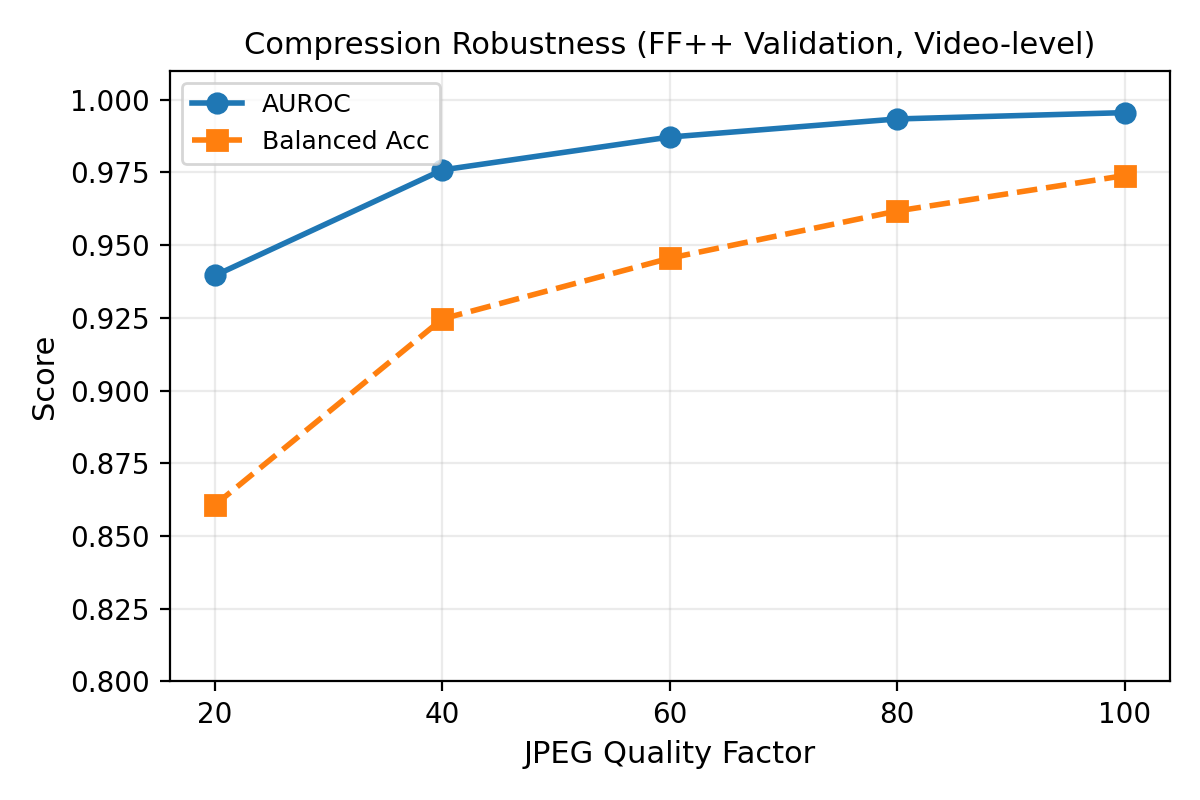
\includegraphics[width=\columnwidth]{figs/jpeg_sweep_ffpp.png}
  \caption{Video-level AUROC and balanced accuracy vs.\ JPEG quality factor on FF++ validation. Performance degrades gracefully under increasing compression.}
  \label{fig:jpeg}
\end{figure}

\subsection{Combined Stress Testing (Compression + Domain Shift)}
To understand how compression and domain shift interact, we repeat the JPEG sweep on Celeb-DF-v2 (Table~\ref{tab:jpeg_cdf}, Fig.~\ref{fig:jpeg_combined}).
At QF=100 the cross-dataset AUROC is 0.897---already 10\,pp below the in-domain value---and it drops to 0.820 at QF=20 (a further 8.6\% relative decline).
Compared to the in-domain sweep (Table~\ref{tab:jpeg}), the cross-dataset curve degrades more steeply and starts from a lower baseline, confirming that domain shift amplifies compression fragility.

\begin{table}[t]
\centering
\caption{JPEG compression robustness on Celeb-DF-v2 (video-level, cross-dataset).}
\label{tab:jpeg_cdf}
\begin{tabular}{ccccc}
\toprule
\textbf{QF} & \textbf{AUROC} & \textbf{AP} & \textbf{EER} & \textbf{BalAcc} \\
\midrule
100 & 0.8972 & 0.9867 & 0.188 & 0.820 \\
80  & 0.8967 & 0.9867 & 0.185 & 0.815 \\
60  & 0.8957 & 0.9865 & 0.192 & 0.810 \\
40  & 0.8835 & 0.9843 & 0.197 & 0.765 \\
20  & 0.8198 & 0.9737 & 0.263 & 0.722 \\
\bottomrule
\end{tabular}
\end{table}

\begin{figure}[t]
  \centering
  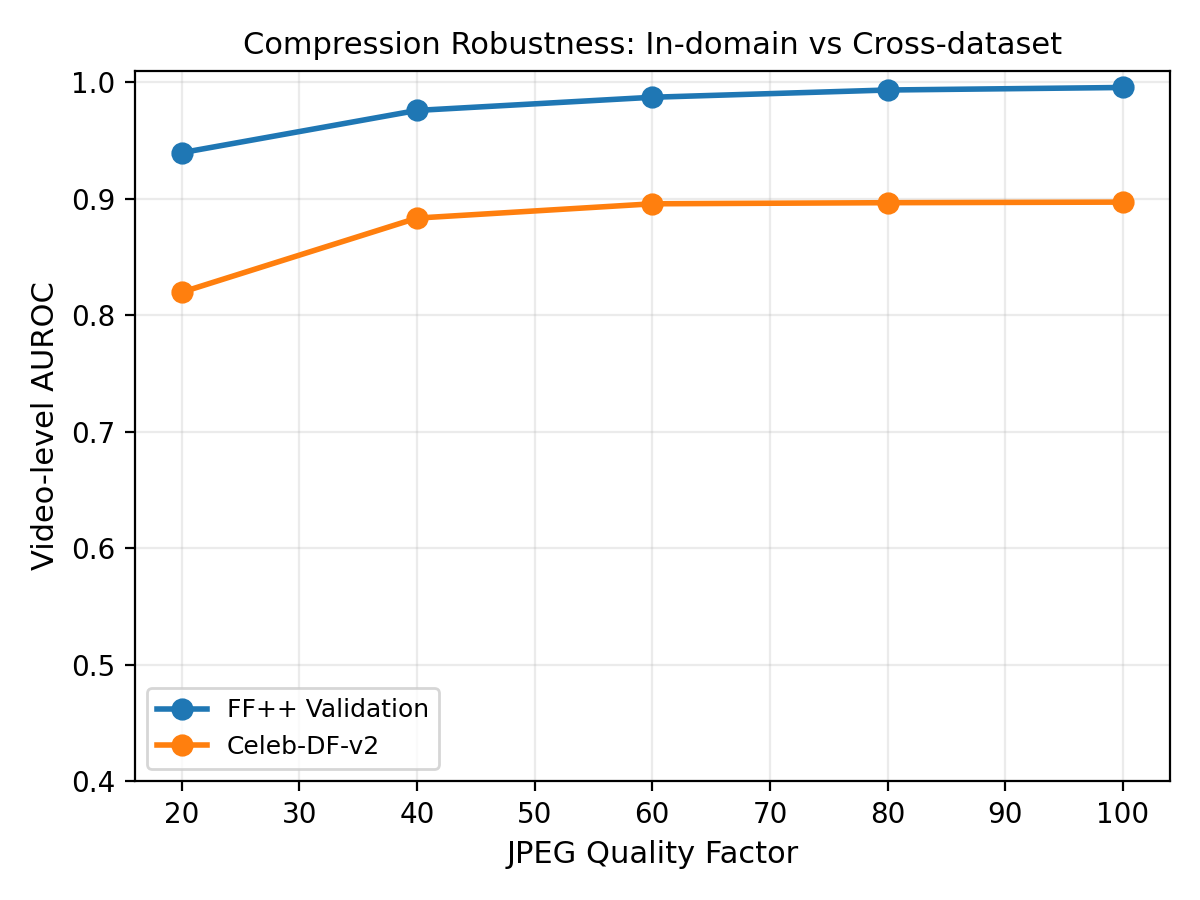
\includegraphics[width=\columnwidth]{figs/jpeg_sweep_combined.png}
  \caption{Video-level AUROC vs.\ JPEG quality factor for both in-domain (FF++ validation) and cross-dataset (Celeb-DF-v2) settings. Domain shift amplifies the effect of compression.}
  \label{fig:jpeg_combined}
\end{figure}

\subsection{Ablation Study}
To isolate the contribution of each stream and the gating mechanism, we evaluate four configurations by manipulating the gate vector at inference time (no retraining):
\begin{itemize}
  \item \textbf{Full model}: learned gate (original).
  \item \textbf{Spatial only}: gate forced to $g{=}1$ (only Xception features).
  \item \textbf{Frequency only}: gate forced to $g{=}0$ (only ResNet-18 DCT features).
  \item \textbf{Average fusion}: gate forced to $g{=}0.5$ (equal weighting).
\end{itemize}

Table~\ref{tab:ablation} reports video-level results on FF++ validation.
The frequency-only stream performs near chance (AUROC\,=\,0.505), confirming that the ResNet-18 DCT branch is insufficient as a standalone detector under these conditions.
However, incorporating frequency features via fusion improves over the spatial-only baseline: both the average fusion (0.9957) and the full model (0.9955) outperform spatial-only (0.9951).
In-domain, the average and learned gates perform comparably; the learned gate's advantage is expected to be more pronounced under compression, where adaptive per-dimension weighting can selectively suppress degraded frequency channels.

\begin{table}[t]
\centering
\caption{Ablation study (FF++ validation, video-level).}
\label{tab:ablation}
\begin{tabular}{lcccc}
\toprule
\textbf{Variant} & \textbf{AUROC} & \textbf{AP} & \textbf{EER} & \textbf{BalAcc} \\
\midrule
Full model    & 0.9955 & 0.9990 & 0.031 & 0.975 \\
Spatial only  & 0.9951 & 0.9989 & 0.034 & 0.971 \\
Freq.\ only   & 0.5046 & 0.8055 & 0.510 & 0.545 \\
Avg.\ fusion  & \textbf{0.9957} & \textbf{0.9991} & \textbf{0.030} & \textbf{0.976} \\
\bottomrule
\end{tabular}
\end{table}


\subsection{Comparison with State of the Art}
Table~\ref{tab:sota} contextualizes our cross-dataset AUROC against published results for FF++$\to$Celeb-DF-v2 generalization.
Direct comparison is complicated by differences in FF++ compression level (c23 vs.\ c40), preprocessing, frame sampling, and whether metrics are frame-level or video-level.
Our model achieves competitive generalization using a simpler two-stream architecture and emphasises transparent operating-point reporting.

\begin{table}[t]
\centering
\caption{Cross-dataset AUC (\%) for FF++$\to$Celeb-DF-v2. Numbers are from respective publications; evaluation protocols vary (c23/c40, frame/video level).}
\label{tab:sota}
\begin{tabular}{lcc}
\toprule
\textbf{Method} & \textbf{Venue} & \textbf{AUC (\%)} \\
\midrule
Xception~\cite{rossler2019faceforensics}   & ICCV'19  & 65.5 \\
F3-Net~\cite{qian2020f3net}                & ECCV'20  & 65.1 \\
Face X-ray~\cite{li2020facexray}           & CVPR'20  & 80.6 \\
Multi-Att.~\cite{zhao2021multiattentional} & CVPR'21  & 67.6 \\
SPSL~\cite{liu2021spsl}                    & CVPR'21  & 76.9 \\
SRM~\cite{luo2021hf}                       & CVPR'21  & 77.5 \\
RECCE~\cite{cao2022recce}                  & CVPR'22  & 68.7 \\
SBI~\cite{shiohara2022sbi}                 & CVPR'22  & 93.2 \\
UCF~\cite{yan2023ucf}                      & ICCV'23  & 82.4 \\
AltFreezing~\cite{wang2023altfreezing}     & CVPR'23  & 89.0 \\
LSDA~\cite{chen2024lsda}                   & CVPR'24  & 93.6 \\
LAA-Net~\cite{nguyen2024laanet}            & CVPR'24  & 95.4 \\
\midrule
\textbf{Ours}                              & ---      & \textbf{90.2} \\
\bottomrule
\end{tabular}
\end{table}

\subsection{Qualitative Analysis: Grad-CAM}
We apply Grad-CAM~\cite{selvaraju2017gradcam} to the final convolutional layer of the Xception spatial stream to visualize which facial regions drive classification (Fig.~\ref{fig:gradcam}).

For fake images, the model consistently attends to regions around the face boundary, jawline, and eye areas---regions where deepfake generators introduce blending artefacts.
For real images, the activation maps are more diffuse and lower in magnitude, indicating that the model does not find concentrated forgery-like patterns.
These observations align with prior findings~\cite{zhao2021multiattentional} that manipulation traces are spatially localized.

\begin{figure}[t]
  \centering
  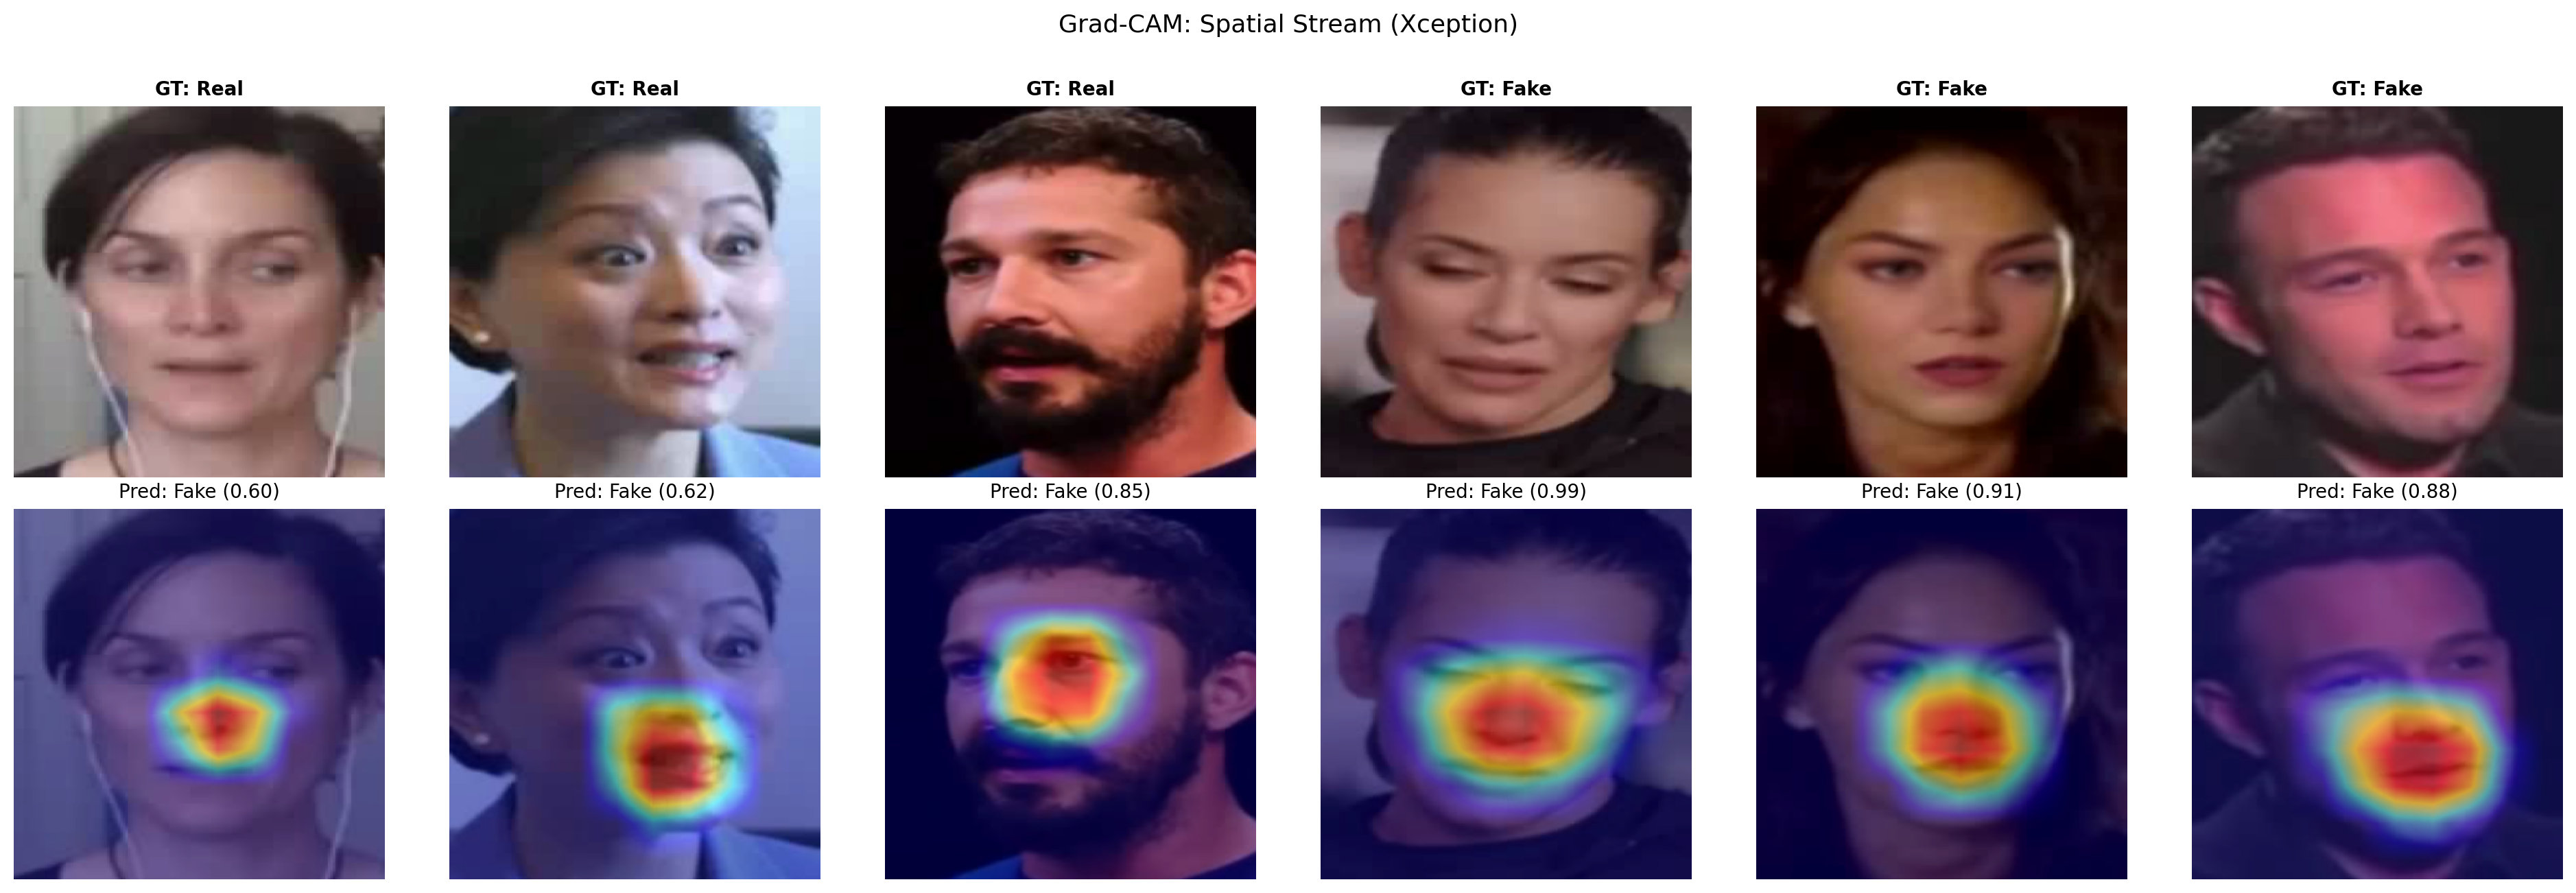
\includegraphics[width=\columnwidth]{figs/gradcam_grid.png}
  \caption{Grad-CAM overlays (Xception spatial stream). Top: original face crops with ground-truth labels; bottom: heatmaps with predicted labels and probabilities. The model focuses on face boundaries and eye regions for fake images.}
  \label{fig:gradcam}
\end{figure}

\textbf{Failure cases.}
The model occasionally misclassifies high-quality real faces with strong lighting contrasts or occlusions (predicted as fake with $p>0.7$), and low-quality fakes with extreme compression artefacts (predicted as real).
These failures suggest that under heavy degradation, the distinguishing cues approach the noise floor.

% ================================================================
% 7. DISCUSSION
% ================================================================
\section{Discussion}

\textbf{Why models fail under compression.}
Lossy codecs destroy high-frequency forensic traces by quantizing DCT coefficients. Our JPEG sweep (Table~\ref{tab:jpeg}) shows that the threshold-free AUROC degrades gracefully, but operating-point metrics (TPR@FPR=1\%) degrade more sharply, indicating that the score distributions overlap increasingly under compression.
The adaptive gate mitigates this by learning to down-weight unreliable frequency dimensions.

\textbf{Domain shift and dataset bias.}
The Celeb-DF-v2 test set has a 9.5:1 fake-to-real ratio, making accuracy at a fixed threshold misleading.
At $\theta{=}0.5$, the model achieves 92.5\% accuracy but only 24.7\% real recall (Table~\ref{tab:operating}), effectively classifying most inputs as fake.
Balanced accuracy and Youden-selected thresholds provide a more faithful assessment.

\textbf{Frequency-domain insights.}
The per-channel DCT representation preserves forensic signatures that differ across RGB channels.
Generator networks introduce colour-channel-dependent spectral artefacts because colour information is often processed at lower spatial resolution in both encoding and generation pipelines~\cite{frank2020leveraging}.

\textbf{Limitations.}
Our evaluation is limited to two datasets (FF++, Celeb-DF-v2). Evaluation on DFDC~\cite{dolhansky2020dfdc}, which includes diverse environmental conditions and lower-quality deepfakes, would provide a more comprehensive assessment.
We do not exploit temporal information across frames; adding a temporal module could improve video-level robustness.

% ================================================================
% 8. CONCLUSION
% ================================================================
\section{Conclusion}

We presented a dual-stream deepfake detector that fuses spatial RGB features with frequency-domain DCT cues through a learned 512-dimensional channel-wise gate.
The architecture, combined with compression-aware training augmentations, achieves strong in-domain performance (video AUROC 0.9955 on FF++) and competitive cross-dataset generalization (video AUROC 0.9018 on Celeb-DF-v2).
Under aggressive JPEG compression (QF=20), the in-domain AUROC degrades to 0.9396---a relative drop of only 5.6\%.
Under combined compression and domain shift (Celeb-DF-v2, QF=20), the model retains an AUROC of 0.820, validating practical robustness.
Ablation experiments confirm that fusing frequency features with the spatial stream improves detection, even though the frequency stream alone is insufficient, and the learned gating mechanism offers a principled adaptive fusion strategy.

\textbf{Future work} includes evaluation on DFDC and WildDeepfake, integration of temporal modelling for video-level reasoning, knowledge distillation to lightweight architectures for edge deployment, and robustness evaluation against adversarial perturbations designed to evade detection.

\section*{Acknowledgment}
We thank our project supervisor Dr.\ Neha Gupta (Delhi Technological University) for guidance and feedback.

\bibliographystyle{IEEEtran}
\bibliography{refs}

\end{document}
